\begin{pastexam}[label={px:ntu-108-ee-dsb-03}]{臺大電機所 108 學年度（B）第 3 題}
（是非；答對 4 分，答錯倒扣 4 分）

There is a min-heap with seven distinct elements so that the preorder traversal of it gives the
elements in sorted order.
\end{pastexam}

\begin{pastsoln}
答案是 (A)，對。

七個節點的完全二元樹是三層全滿的樹。 前序走訪的順序是「根、左子樹、右子樹」（資結書
第~7.3~節），所以只要把 $1, 2, \ldots, 7$ 照前序走訪的順序填進去：
\begin{center}
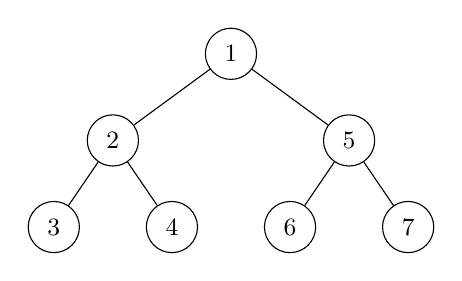
\begin{tikzpicture}[
    every node/.style={circle, draw, minimum size=6.5mm, inner sep=0pt, font=\small},
    level 1/.style={sibling distance=30mm, level distance=11mm},
    level 2/.style={sibling distance=15mm, level distance=11mm}]
\node {1}
    child {node {2} child {node {3}} child {node {4}}}
    child {node {5} child {node {6}} child {node {7}}};
\end{tikzpicture}
\end{center}
前序走訪：先訪根 $1$；再走左子樹，依序 $2, 3, 4$；最後走右子樹，依序 $5, 6, 7$。 得到
$1, 2, 3, 4, 5, 6, 7$，由小到大。

檢查最小堆積的條件（父節點小於子節點）：$1 < 2$、$1 < 5$；$2 < 3$、$2 < 4$；$5 < 6$、
$5 < 7$。 全部成立，形狀也是完全二元樹，所以這是一個合法的最小堆積。

一般來說，前序走訪時父節點一定比它的子孫先被訪問，而最小堆積要求父節點比子孫小，兩個要求方向
一致，所以「照前序順序填 $1..n$」總是得到最小堆積。 用陣列寫出來就是
$A = \langle 1, 2, 5, 3, 4, 6, 7\rangle$，而且七個不同的數裡只有這一種填法。
\end{pastsoln}
